\chapter{Gamma spectrum software analysis}
As mentioned in section \ref{char}, the measured gamma spectrum contains many unwanted artefacts such as noise, Compton continuum and edges, and additional peaks caused by various interactions. To correctly obtain the count rates at defined energies, it is necessary to perform a numerical analysis of the measured data. Locations of energy peaks are found, for example, by their characteristic second derivatives. Absolute count rates are then obtained by Gaussian fitting.
%As was mentioned before in section \ref{char}, the measured gamma spectrum contains many unwanted artifacts like noise, Compton continuum and edges and additional peaks created by various interactions. To properly obtain the count rates at defined energies, it is necessary to perform a numerical analysis of measured data. Locations of energy peaks are found for example by their characteristic second derivatives. Absolute count rates are then obtained by Gaussian fitting.


\section{Peak searching procedure}
\label{search}
Many commercial programs use peak search procedures based on an algorithm originally developed by M.A. Mariscotti \cite{MARISCOTTI1967309}. This method is based on the numerical second difference, which assumes that the background can only be approximated by linear functions and therefore vanishes in the second derivative. The second fact is that the searched peaks are Gaussians with their specific second derivatives and thus their positions can be found in local minima (Gaussians have negative second derivatives as they are concave functions). To reduce noise, the second difference is averaged over a defined number of steps. Rules based on the value of the standard deviation of the second difference at a given point and other additional rules based on the number of points in specified intervals can be used to determine whether the found minimum should be considered as a peak position (and not as a Compton edge, etc.). However, the algorithm requires input parameters based on a raw estimation of the FWHM of the searched peaks.
\par
For the analysis of measured gamma spectra, this algorithm was implemented in C++ and used to find peaks and edges. The following figures \ref{Example} and \ref{secondDerivative} show the example of measured spectra and their second difference plotted together with their calculated standard deviation. The possible candidates for peak positions can be observed.
%Many commercial programs use peak searching procedures based on algorithm originally developed by M.A. Mariscotti \cite{MARISCOTTI1967309}. This method is based on the numerical second difference assuming that the background can be approximated only by linear functions and thus it vanishes in case of the second derivative. The second fact is that the searched peaks are Gaussians with their specific second derivatives and thus their positions can be found in local minimums (Gaussians have negative second derivatives since their are concave functions). To reduce noise, the second difference is averaged by defined number of steps. To determine if the found minimum should be considered as peak position (not as a Compton edge etc.), rules based on the value of standard deviation of second difference at given point and other additional rules based on number of points in specified intervals can be employed. However, algorithm needs input parameters, which are based on raw estimation of FWHM of searched peaks.
%\par
%For the analysis of measured gamma spectra, this algorithm was implemented in C++ and used to find peaks and edges. The following figures \ref{Example} and \ref{secondDerivative} show the example of measured spectra and its second difference plotted along with its calculated standard deviation. The possible candidates onto peak positions can be observed.



\begin{figure}[H]
 \centering
 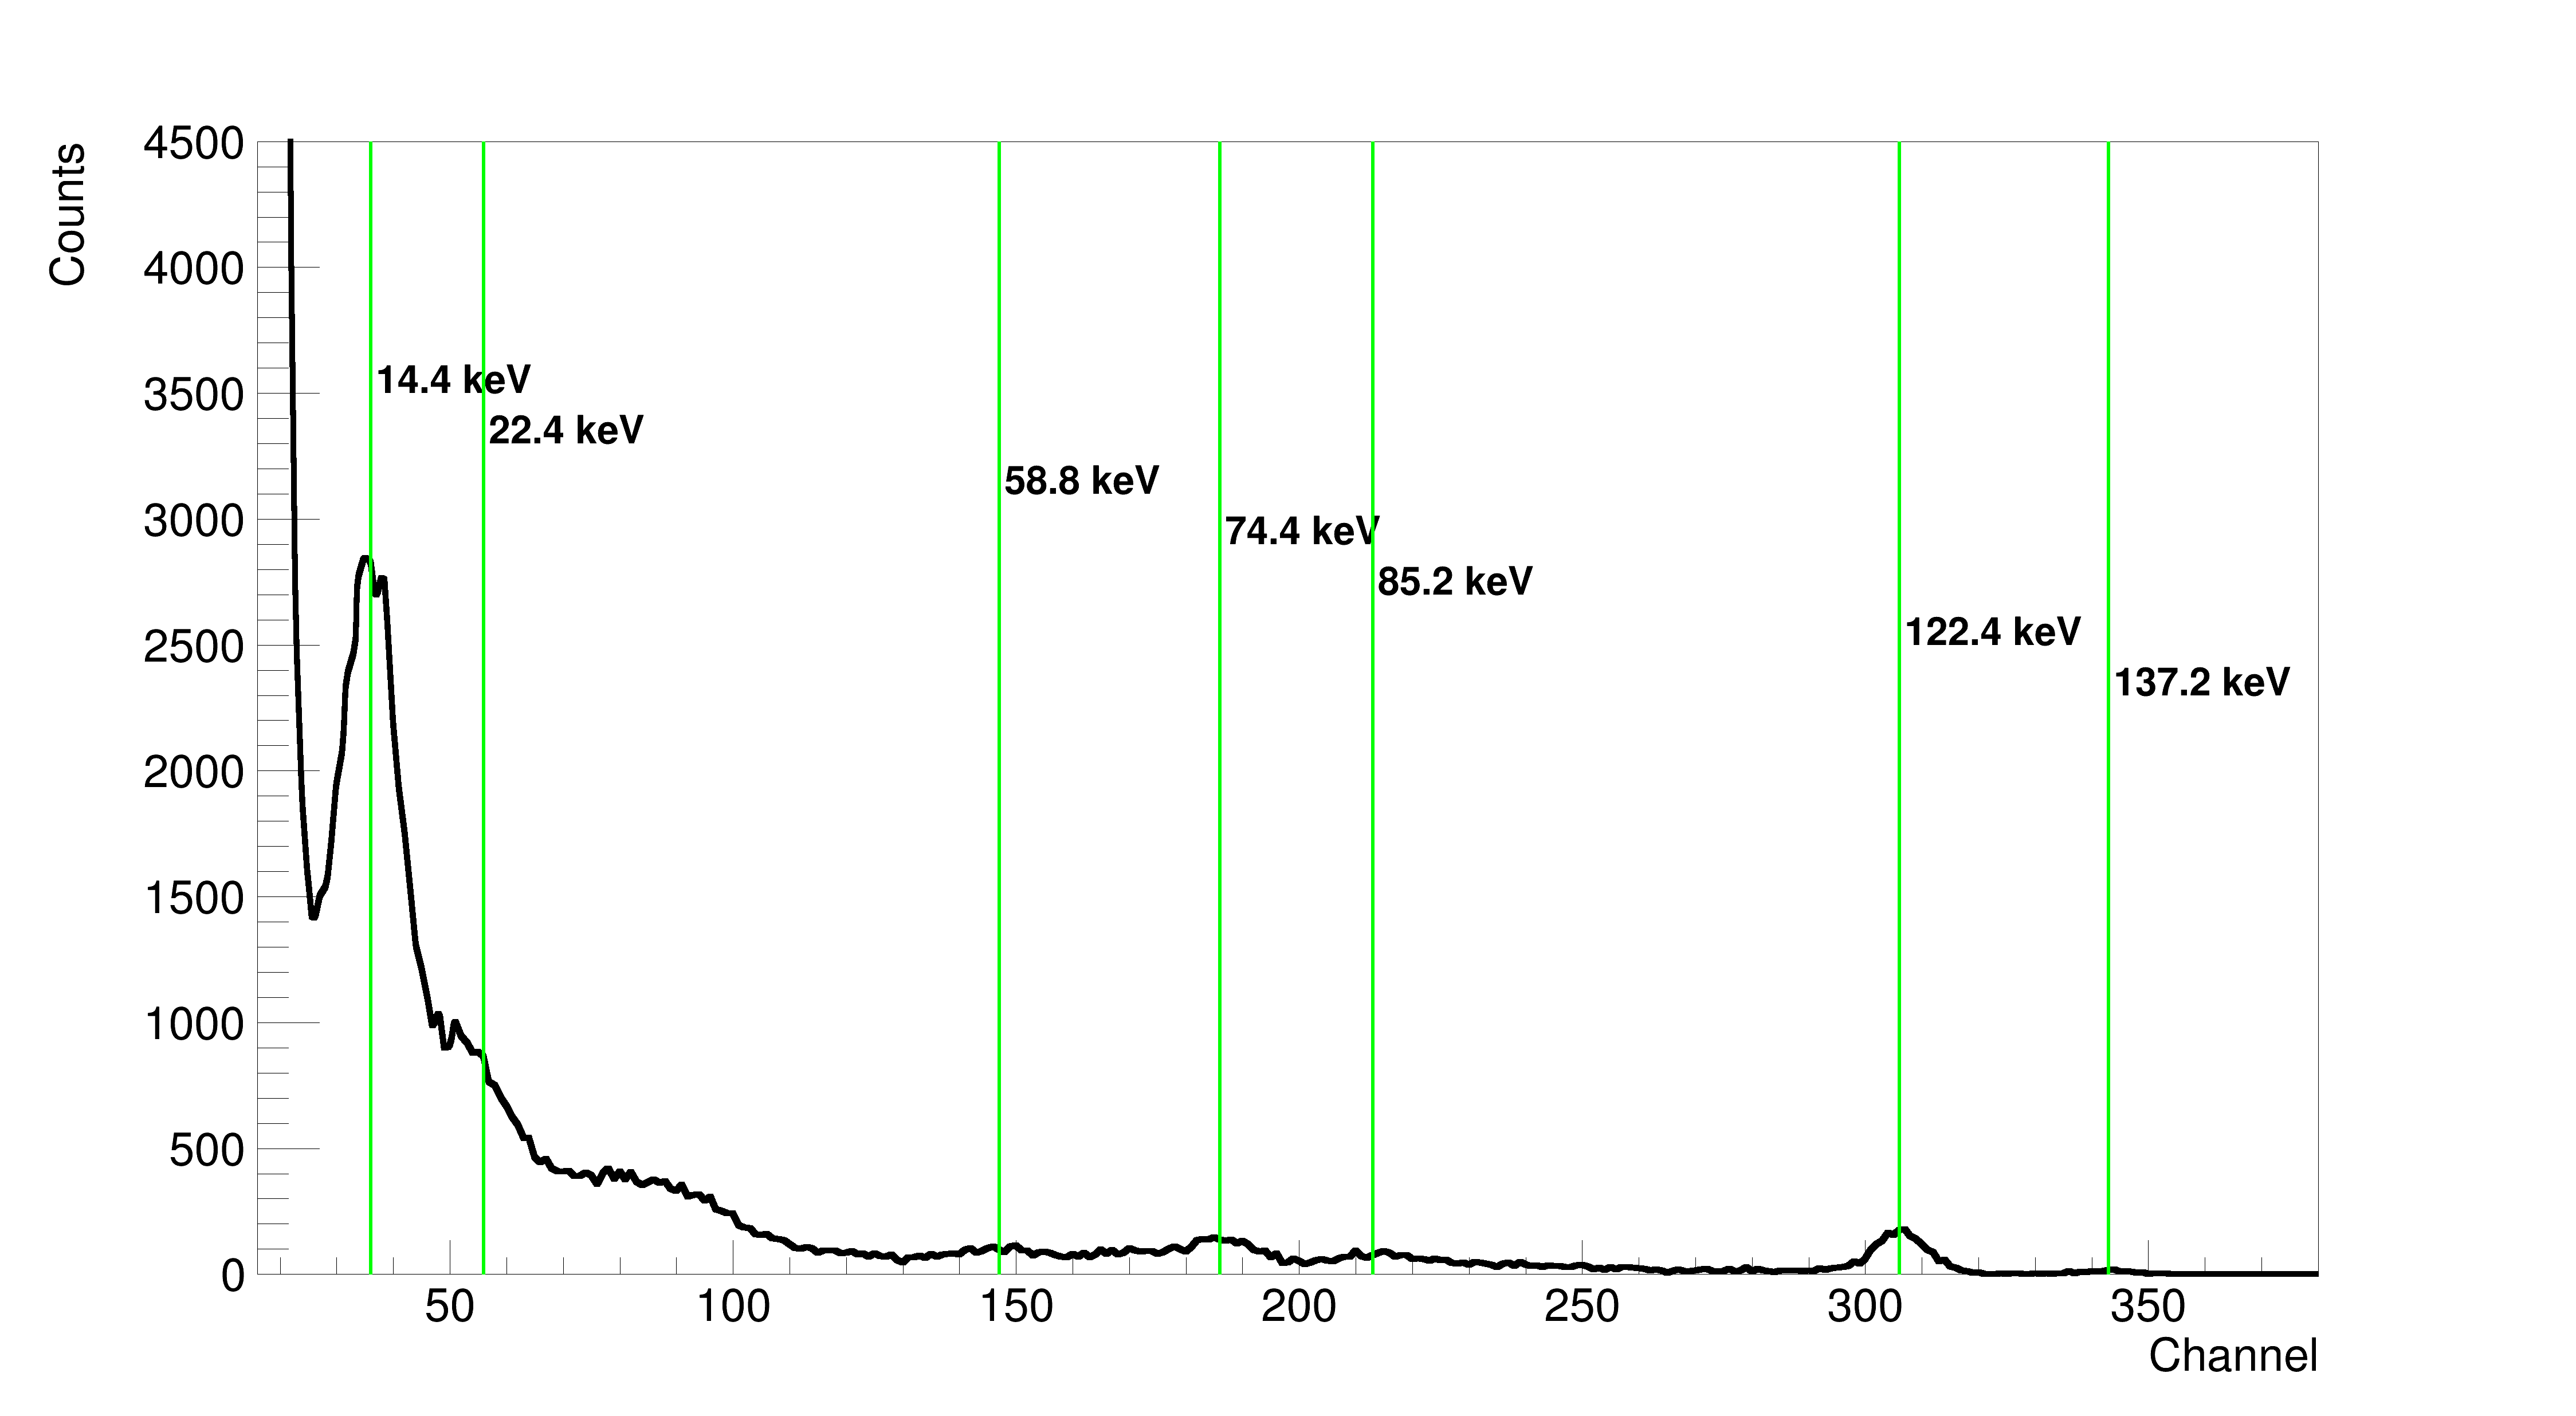
\includegraphics[scale=0.105, angle = 0]{./pictures/DataGraph.png}
 \caption{Example of measured gamma spectra. Green lines mark the energy peaks found by algorithm.}
 \label{Example}
 
\end{figure}

\begin{figure}[H]
 \centering
 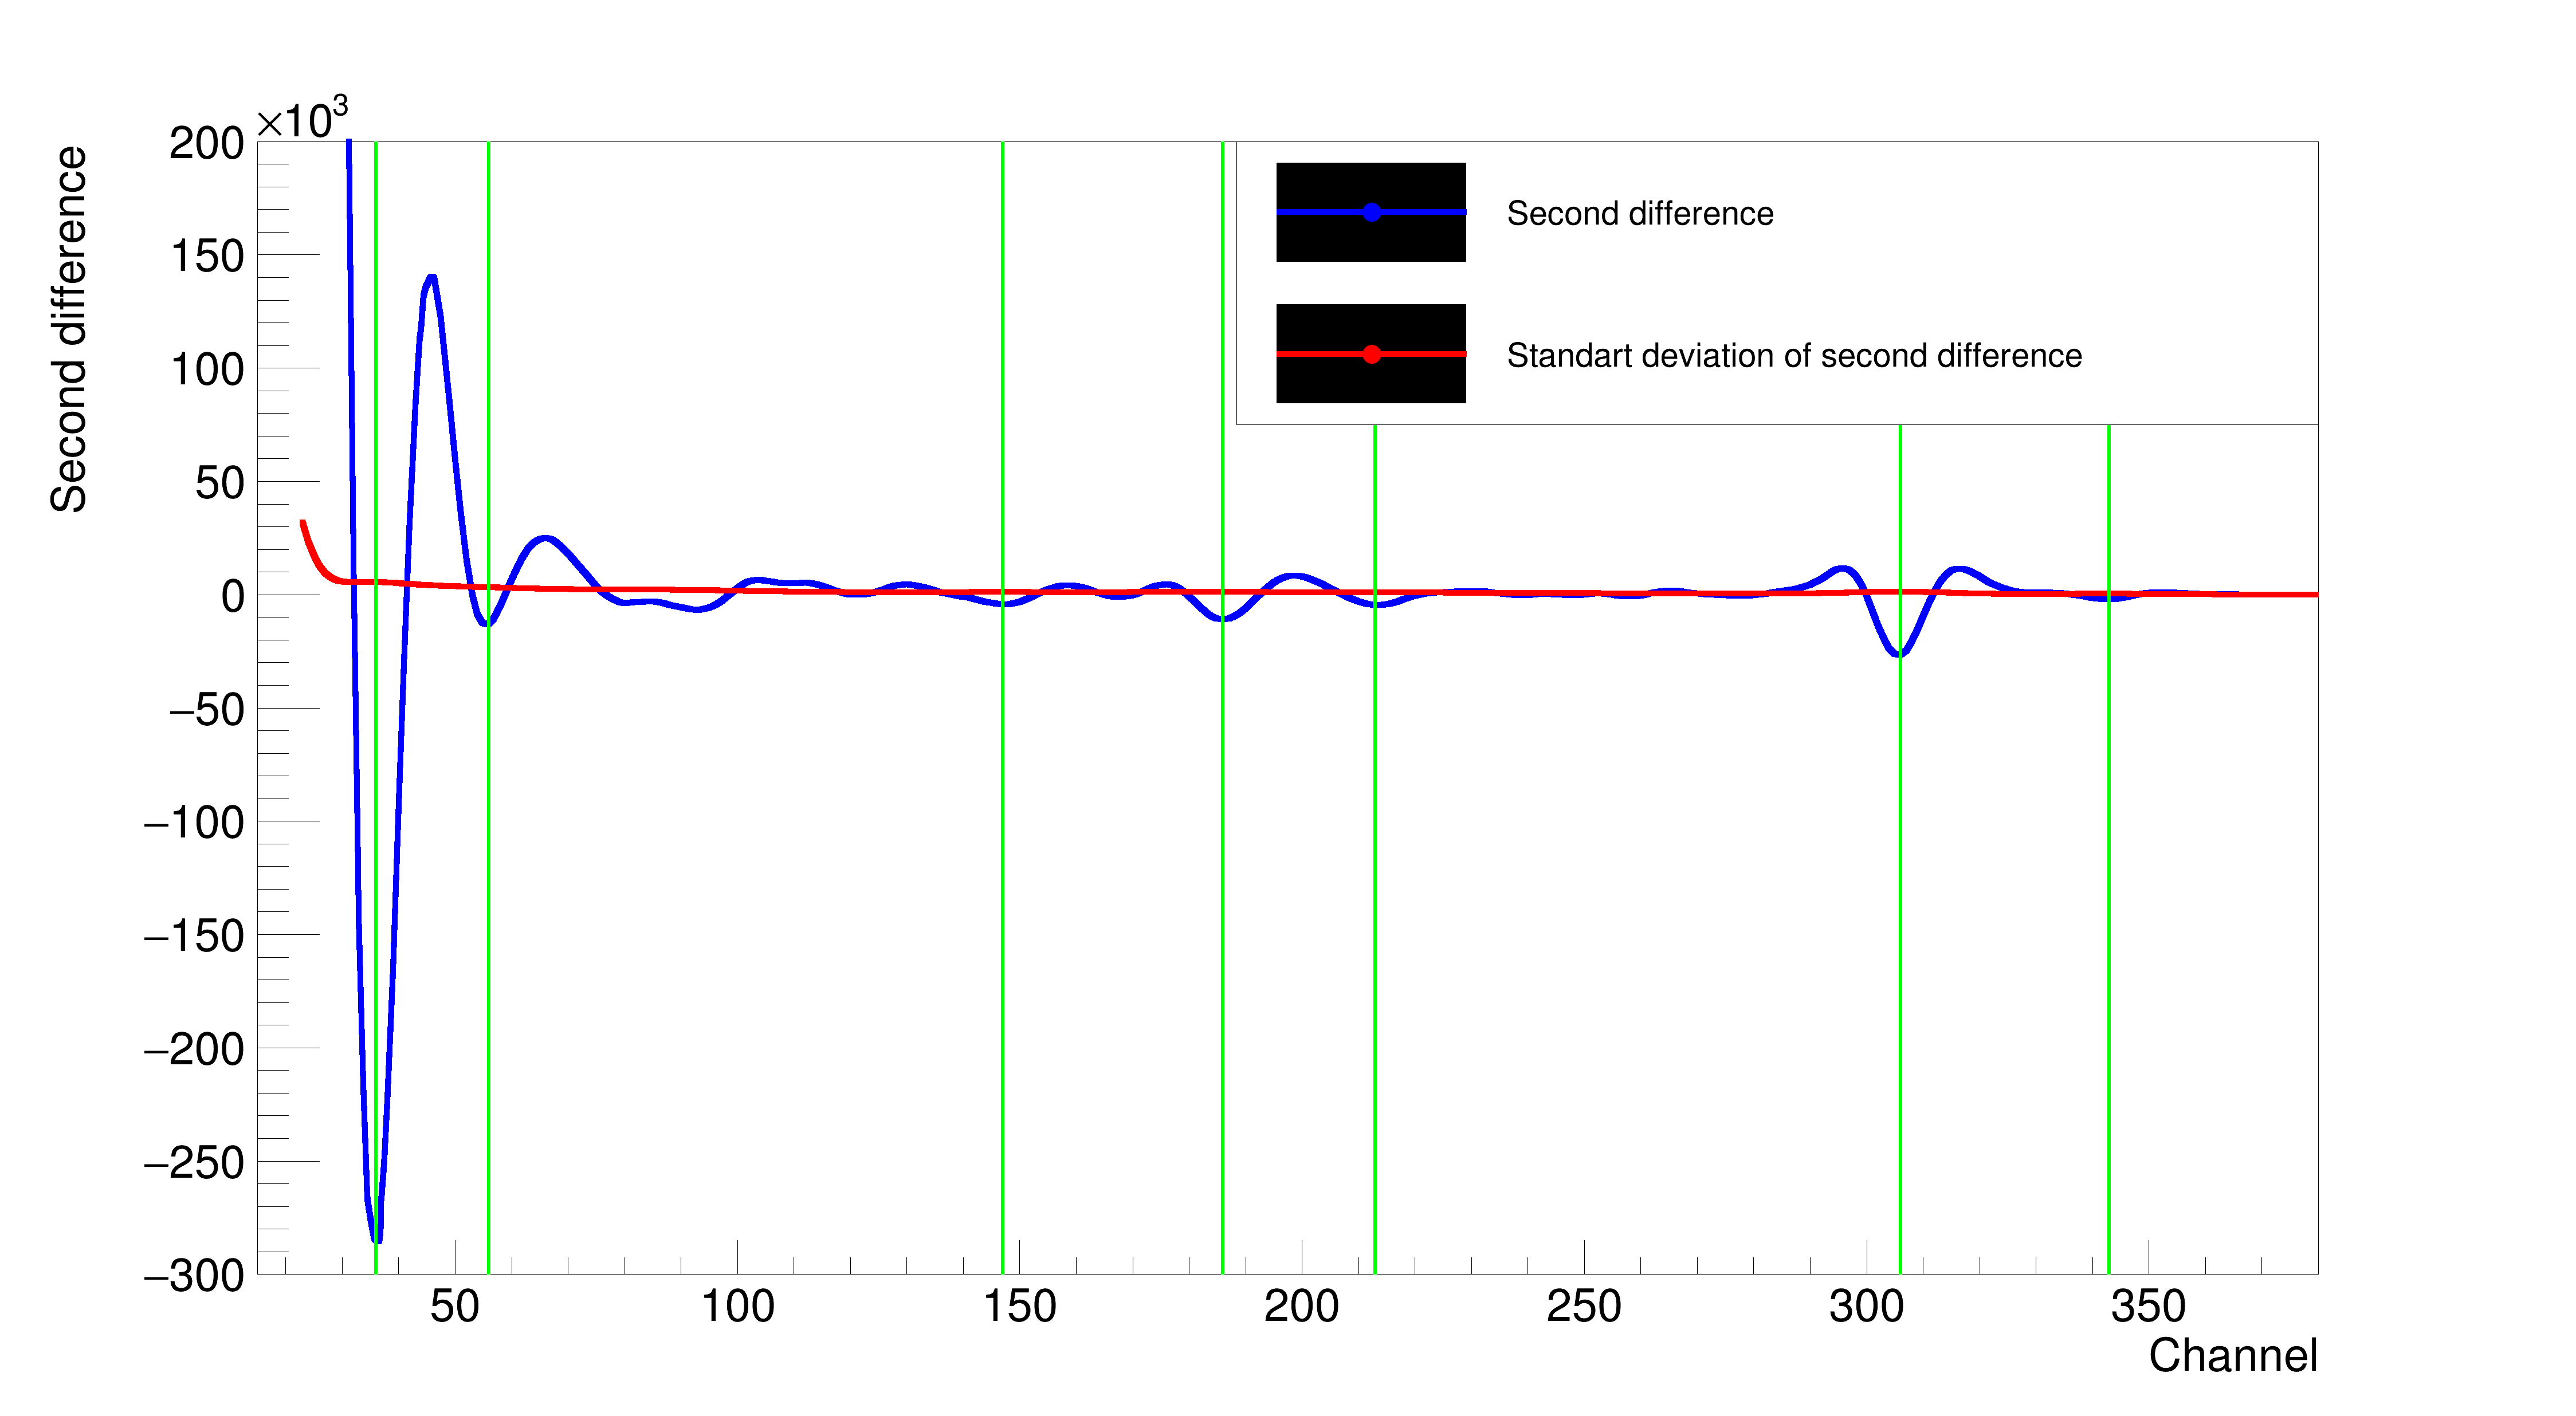
\includegraphics[scale=0.105, angle = 0]{./pictures/SecondDerivGraph.png}
 \caption{Second difference of example spectra along with its standard deviation showing possible candidates (green lines).}
 \label{secondDerivative}
 
\end{figure}


